%-----------------------------------------------------------------------------------------------
%		\COMPdataFormatManagement{} Design
%-----------------------------------------------------------------------------------------------

\section{\COMPdataFormatManagement{} Design}
\label{sec:COMPdataFormatsDesign}

In this section, the design of the component \COMPdataFormatManagement{} is described. Basic task of the component is to describe the structure of a container or metadata format in a way that is useful for parsing them generically.

% =======================================================================================================
\subsection{Format Comparison}%
\label{sec:FormatComparison}%

Before any real design decisions can be found, we have to look what the formats are that we try to generically describe with the \COMPdataFormatManagement{} component. The main source of this whole chapter is \cite{MC17}.

We fully focus on the following data formats here, ignoring any other possible formats as out of scope:
\begin{itemize}
\item Multimedia container formats: Ogg, QuickTime, MPEG Layer I Elementary Stream (for MP3), Matroska, RIFF
\item Metadata container formats: ID3v1 and ID3v1.1, ID3v2.2, ID3v2.3, ID3v2.4, VorbisComment, Lyrics3v1, Lyrics3v1, APEv1 and APEv2
\end{itemize}

As first introduction, we have to compare those formats according to their most important structural aspects. These aspects are as follows:
\begin{itemize}
\item Basic encoding they use: \textbf{Byte orders} and \textbf{character encodings} supported
\item Building blocks: What are the \textbf{containers} in this format? Are there other sub-structures? Can they be embedded in each other? Is there a hierarchical structure with arbitrary nesting? For metadata container formats, we call the elements actually holding the metadata \emph{attributes}, which is nothing else than a special case of a container.
\item Headers and Footers: Despite the payload, are there \textbf{headers} and/or \textbf{footers} in the containers or attributes? Are they fixed or variable size?
\item Lengths of containers: How is the \textbf{length of containers} or of their payload defined?
\item Lengths of attributes: How is the \textbf{length of attributes} for metadata container formats defined?
\item Padding: Does the format have some special way of supporting \textbf{padding}?
\end{itemize}

The following table provides all these properties for multimedia container formats, skipping attribute topics:

TODO Table for multimedia formats
tab:DFcompareMult

The following table compares these properties for the metadata container formats considered:

TODO Table for metadata formats
tab:DFcompareMeta

Note that ID3v2x is a very special format in multiple dimensions: It is incredibly overloaded with a lot of features you might never dare dream to use, say: over-designed. It offers e.g. support for encryption, grouping, compression of tags, embedded lyrics or audio guide codec data which basically contain spoken versions of the metadata stored and other things. On top of that, it has a strange conversion scheme called the \emph{unsynchronization scheme}. 

% =======================================================================================================
\subsection{The Container Metamodel}%
\label{sec:TheContainerMetamodel}%

In order to give a feasible model of the structure of a container format (which includes metadata container formats), a metamodel of the typical data structure of a container format is developed here. 

The metamodel is ultimately shown in the following figure, the corresponding design decisions will follow:

\begin{figure}[htbp]
\centering
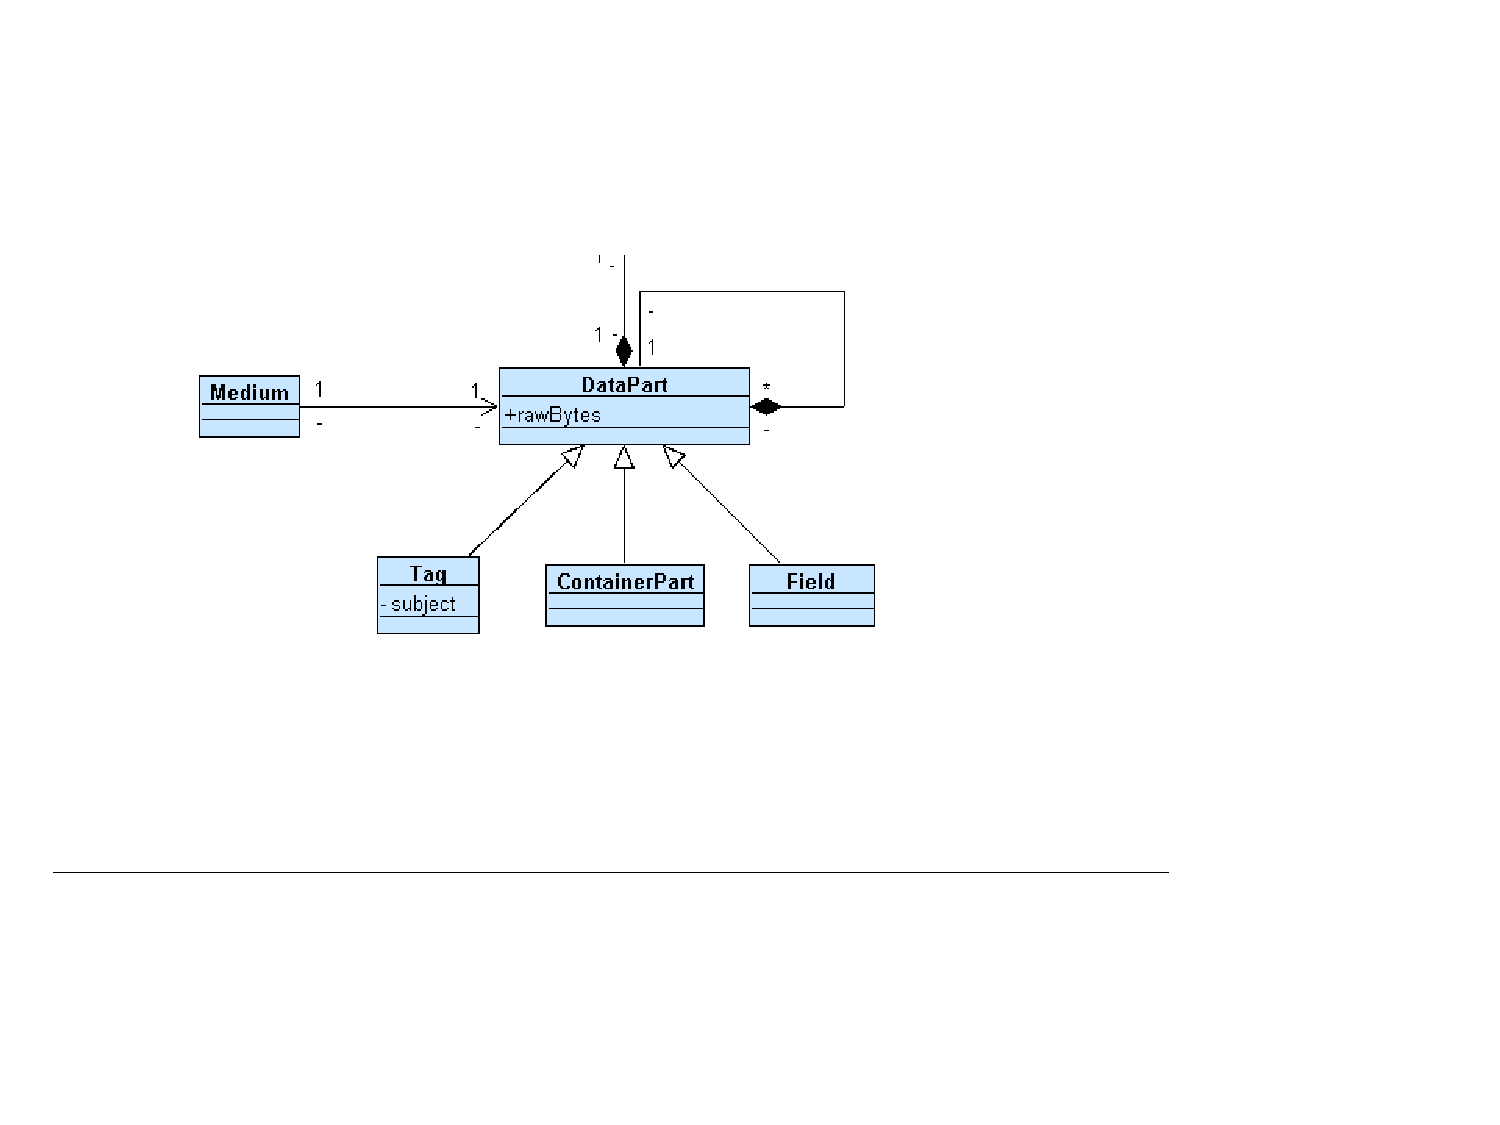
\includegraphics[width=1.00\linewidth]{figures/II_GeneralModel.pdf}
\caption{The container metamodel}
\label{fig:II_GeneralModel}
\end{figure}

%%%% DD --> %%%%
\DD{dd:500}
{% Title
Containers as basic top-level unit, containing nested containers
}
{% Short description
All data that can be processed by \LibName{} consists of containers. A container is a sequence of bytes with a specific structure belonging to exactly one container data format. However, consecutive containers might belong to different data formats.

In addition, a container - as the name suggests - contains other data. This data might be containers of the same format again. The nesting might be arbitrarily deep. A nested container is able to contain data of other formats. 
}
{% Rationale
Every format considered here has such basic building blocks, called differently in each format specification (atom, frame, page, element, item, tag etc.). The same file or media stream might consist of containers belonging to different formats. One example is an MP3 file with an ID3v2 tag. See also \cite{MC17}, part IV for more details.

Most of the supported data formats have some notion of nesting child containers (or, for metadata formats: attributes) within parent containers. Those child containers have either exactly the same stucture as the top-level containers, or they differ slightly. Some formats such as RIFF explicitly define specific containers that embed data belonging to other metadata formats. 
}
{% Disadvantages
No disadvantages known
}
%%%% <-- DD %%%%

How are these containers structured in detail?

%%%% DD --> %%%%
\DD{dd:501}
{% Title
A container consists of an optional \textbf{header}, \textbf{payload} and an optional \textbf{footer}
}
{% Short description
Every container - no matter which data format - follows the same basic structure: One or more optional headers start the container's byte sequence. Following this, there is a sequence of bytes called the payload. At the end of the container, there are one or more optional footers. A container must either have at least a single header or at least a single footer.
}
{% Rationale
Considering table \ref{tab:DFcompareMult} and \ref{tab:DFcompareMeta}, every container in every format has at least one header or one footer, including nested containers. Only ID3v23 as sole exception has a second, so-called extended header. Thus we have to support multiple headers and footers, even though this might be a singular case. But future formats might come to bring multiple headers, too. Modelling the middle part of a container as payload explicitly instead of just as list of sub-containers or fields makes sense because it allows to lazily read substructures, or entirely skip the payload.
}
{% Disadvantages
No disadvantages known
}
%%%% <-- DD %%%%

We saw that containers have a structure, and containers can live within other containers. But on the lowest level, there are leaf nodes, the fields:

%%%% DD --> %%%%
\DD{dd:502}
{% Title
Fields as the atomic unit of all byte sequences
}
{% Short description
\textbf{Field}s are the leaf nodes of the container metamodel: A field is a sequence of 1 to N consecutive bytes. A field has a \textbf{binary value} as well as an \textbf{interpreted value}, i.e. a human-understandable value with a specific meaning. We say that a field has a specific type, which basically describes the mapping between binary and interpreted value as well as the allowed values or format of a field.
}
{% Rationale
The term ``field'' is quite commonly used in binary data formats. It does not make sense to go down to individual byte or bit level. The smalles level of semantic in every binary or textual format is a field.
}
{% Disadvantages
No disadvantages known
}
%%%% <-- DD %%%%

Now towards headers and footers: Are they inherently different or basically the same? Fixed or variable size?

%%%% DD --> %%%%
\DD{dd:503}
{% Title
Headers and footers as sequences of fields are structurally identical
}
{% Short description
Headers and footers are sequences of fields, i.e. they must not nest a container. They are either variable or fixed-size. For both header and footer, the same model class called FieldSequence is used.
}
{% Rationale
No data format specifies a header or footer nesting a container-like data structure, they all consist of plain fields. Despite the location (before or behind the payload), there is nothing really distinguishing headers or footers from a structural perspective. Thus the same model class can be used for both. However, there is no english term for that class that seems to clearly be a grouping term for headers and footers.
}
{% Disadvantages
No disadvantages known
}
%%%% <-- DD %%%%

So far, we just introduced containers, fields, headers, footers and payload. We learned that containers might embed other containers, while headers and footers must only consist of fields. But what about the structure of the payload of a container? Of course, if the headers and footers cannot embed child containers, they must hide within the payload. Is this the only possibility? Of course not:
%%%% DD --> %%%%
\DD{dd:504}
{% Title
Payload either solely consists of containers or fields
}
{% Short description
The payload of a container either fully consists of a sequence of child containers or of a sequence of fields, but never both.
}
{% Rationale
Ultimately, we must boil payload down of fields, or put otherwise: We cannot recurse indefinitely into sub-containers. So at last, there must be a final sequence of child containers having payloads solely consisting of fields. So it is clear that we have both cases. But what about the mixed case: Should we have containers in the model that have both child fields neighbouring child containers? In rare cases such as - again - ID3v2, it would be possible to think of having the frames as child containers of the tag, followed by the padding child field of the tag behind it. However, we avoid such complexities, but payload is either ContainerBasedPayload or FieldBasedPayload. See next design decision of how we handle the ID3v2 special case.
}
{% Disadvantages
No disadvantages known
}
%%%% <-- DD %%%%

How to handle padding? If we look at the data format comparisons in \ref{tab:DFcompareMult} and \ref{tab:DFcompareMeta}, we see that padding is just a special case in ID3v2 and MP3. All other formats solve it ``more naturally'' by embedding it in special child container. ID3v2 just adds some nullbytes at the end of the tag payload behind the frames. How to model this? There are basically three possibilities:
\begin{itemize}
\item The padding is a part of the payload, basically a field. This seems most intuitive, but is already excluded by the previous design decision, because then we would need to support mixed payloads, consisting both of child containers and fields.
\item The padding is part of the payload, but considered as a very special child container.
\item The padding is an optional part of the tag footer.
\end{itemize}

Based on these alternatives, we can really only decide the following:
%%%% DD --> %%%%
\DD{dd:505}
{% Title
Padding in ID3v2 is modeled as very special child container of the tag
}
{% Short description
Padding in ID3v2 is modeled as very special child container of the tag, where the header is the first null byte, and all follow-up bytes form the payload. 
}
{% Rationale
Modeling it as child field of the payload is not possible as it would contradict \DesLink{dd:504}. Modeling as part of the footer would be odd, as not every version of ID3v2 defines a footer at all, and we would have a variable sized footer optionally starting with an arbitrary number of nullbytes, which would not be very intuitive from a library users perspective, too.
}
{% Disadvantages
The only disadvantage possibly to be identified that there could be padding just consisting of a single byte. This would mean we'd have a container with just a header, but an empty payload, which actually is quite degenerate.
}
%%%% <-- DD %%%%

The overall term for containers, headers, footers, fields and payload is a \textbf{datablock}. This term is used further on throughout this document.

There is another ID3v2 specific that we directly want to exclude here:
%%%% DD --> %%%%
\DD{dd:505b}
{% Title
ID3v2 transformations such as unsynchronization, compression, encryption are not handled generically
}
{% Short description
ID3v2 is clearly overdesigned. It includes an outdated mechanism called \emph{unsynchronization} to ensure players do not interpret ID3v2 tags as MP3 frames and try to play them. ID3v2 also defines frame-based compression and encryption possibilities.

These facilities are not handled generically in \LibName{}, they are just specifically implemented in the ID3v2 extensions.
}
{% Rationale
Unsynchronization is not needed anymore, as current players all know about ID3v2 tags. Even if it would be needed: There is no other data format know to date that defines any such transformation schemes, not even for compression or encryption.

Thus, declaring this all as generic concept is useless as only one format defines such things, and these things are even only very rarely used.
}
{% Disadvantes
No disadvantages known
}
%%%% <-- DD %%%%

% =======================================================================================================
\subsection{Representing a Data Format}%
\label{sec:RepresentingaDataFormat}%

Data Formats need some kind of representation:
%%%% DD --> %%%%
\DD{dd:506}
{% Title
Class for data formats and especially for container formats
}
{% Short description
There is a base class called \texttt{AbstractDataFormat} representing a general data format, which has a subclass called \texttt{ContainerDataFormat} that is used for all data formats listed in \SectionLink{sec:FormatComparison}. Each individual format is represented as an instance of \texttt{ContainerDataFormat}. These two classes are neither enums nor ``dynamic enums'', but just plain old java classes.
}
{% Rationale
We need some way to identify which data format a container belongs to. A class allows to store additional format-wide properties for logging or even with a functional notion behind. Why not using an enum to identify each supported data format? Because enums are static, and we do not want to change the enum whenever a new format comes around. And it is not clear which formats are out there by 3rd party. A dynamic enum pattern is unnecessarily complexity here, so just a plain class. Why a just an instance of \texttt{ContainerDataFormat} rather than a new subclass for each format supported? First of all, data formats must be used as tokens by end-users of the library to refer to which tags or containers they want  to read. Creating a new sub-class instance everytime they want to have a token is strange. Instead, they can use a public constant instance as token. The next question: Why at all a \texttt{ContainerDataFormat} subclass? The reason is that \LibName{} might want to support even more different formats in future, e.g. XML. This can be a sibling subclass of \texttt{AbstractDataFormat}. From now on, everything described in this section is only covering container data formats.
}
{% Disadvantes
No disadvantages known
}
%%%% <-- DD %%%%

But that's not all of it. If we structure data belonging to a format into containers, headers, footers and so on according to the generic metamodel, \emph{how exactly} is a correct datablock of a given format structured? Of course, each format individually specifies the exact structure of its containers (how many headers, footers etc., what the payload can contain), headers (which fields make up a header), fields (which type a field has, how long it is and which values it can have) and so on. Thus, we need a place where we describe the structure of all datablocks belonging to a data format in more detail, otherwise we could not parse this data generically.

We define:
%%%% DD --> %%%%
\DD{dd:507}
{% Title
\texttt{DataFormatSpecification} provides \texttt{DataBlockDescription}s, \texttt{DataFormatRepository} maintains all \texttt{DataFormatSpecification}s
}
{% Short description
The exact properties of a datablock is described by an instance of the class \texttt{DataBlockDescription}. Which properties are needed in detail is determined later in \SectionLink{sec:DatablockProperties}.
The interface \texttt{DataFormatSpecification} provides access to all \texttt{DataBlockDescription}s offered by one specific data format. Last but not least there is a \texttt{DataFormatRepository} interface which basically only maintains a list of all supported data formats and their corresponding \texttt{DataFormatSpecification}s.

A concrete \texttt{DataFormatSpecification} is defined in an extension and loaded when starting \LibName{}. 
}
{% Rationale
For generically parsing data blocks according to a format definition, the parser code needs information about the exact structure of a data block. Thus, we need a place to maintain all data formats, their specifications and a description of each possible individual container, field etc.
}
{% Disadvantes
No disadvantages known
}
%%%% <-- DD %%%%

% =======================================================================================================
\subsection{\texttt{DataBlockDescription} Common Properties}%
\label{sec:DatablockProperties}%

First of all, we need a clear way to identify each specific datablock that might occur in the data format. Every container type, header, footer, field and payload needs an identifier:
%%%% DD --> %%%%
\DD{dd:508}
{% Title
Each datablock of a format has a specification id unique across all supported formats
}
{% Short description
Each distinctly defined container, header, footer, field or payload block of a data format is assigned a unique specification id. Using this specification id, a parser implementation can lookup the \texttt{DataBlockDescription} of the block from its associated \texttt{DataFormatSpecification}. Specification ids are human-readble rather than generated GUIDs. The uniqueness is guaranteed by using a top-level prefix identifier that is directly checked to be unique upon all loaded data formats when loading the extension defining the data format. The ids reflect the hierarchical nature of a data format according to the container meta model, following these rules:
\begin{itemize}
\item Each id consists of one or more \emph{segments} separated by a dot.
\item A segment name does only contain ASCII alphanumeric characters, starting always with a lower-case letter and preferring lower-case only letters, i.e. no special characters, no blanks etc. So a datablock id has much in common with a Java package name. 
\item The first segment is the data format top-level prefix which equals the (single) top-level container id of the data format. So we have the implicit decision that each format starts off with a single container on top-level enclosing everything else. This is true for all data formats considered here.
\item Each container consists of an arbitrary number of headers and footers as well as exactly one payload. The segment name of a container payload is always \texttt{payload}. If there is just a single header or footer, it is called header or footer respectively. Multiple headers or footers bear more specific, distinct names.
\item Child fields of a header or footer have descriptive names and so on 
\end{itemize}
}
{% Rationale
When parsing, the format structure of a datablock must be clearly visible and available. By an id, this format structure is clearly adressable and the corresponding \texttt{DataBlockDescription} can be obtained from a \texttt{DataFormatSpecification}. The uniquenss of the id guarantees that the parsing logic cannot unintentially try to parse a block of bytes according to the incorrect format.

The reason for not using generated unique ids such as counters or GUIDs is that we want to have memorable and recognizable names, both for library developers (e.g. during debugging) or \LibName{} end-users that need to work with datablock ids directly. 
}
{% Disadvantes
No disadvantages known
}
%%%% <-- DD %%%%

Besides their id, what else might be desirable on first glance when looking at a datablock taken from a data format's specification? Some descriptive stuff comes to mind. Second, it seems like every datablock must have exactly one type that is useful to store. So we can state:
%%%% DD --> %%%%
\DD{dd:509}
{% Title
Basic properties held in a \texttt{DataBlockDescription}
}
{% Short description
Each \texttt{DataBlockDescription} instance holds the datablock id of the datablock according to \DesLink{dd:508}. In addition, it has:
\begin{itemize}
\item A more human-readable name of the datablock, if available; only for display or documentation purposes
\item A description of the datablock, probably taken from the format specification, preferably in English. This is meant to give more information about the purpose of the datablock, but has no other meaning.
\item The \texttt{DataBlockType} of the datablock, which is: \texttt{HEADER}, \texttt{FOOTER}, \texttt{CONTAINER}, \texttt{FIELD}, as well as \-- according to \DesLink{dd:504} \-- \texttt{FIELD\_BASED\_PAYLOAD} or \texttt{CONTAINER\_BASED\_PAYLOAD}.
\end{itemize}
}
{% Rationale
These properties are clear from the beginning, the concrete is known statically, and it is needed to take decisions during generic parsing. 
}
{% Disadvantes
No disadvantages known
}
%%%% <-- DD %%%%
 
We defined that datablock ids are organized hierarchically as their real blocks are organized hierarchically. However, still, it is not sufficient to somehow maintain the ``hierarchy'' indicated by the metamodel only in the datablock ids. Instead, we define:
%%%% DD --> %%%%
\DD{dd:510}
{% Title
\texttt{DataBlockDescription}s contain a list of all child ids they might contain, where order matters
}
{% Short description
A \texttt{DataBlockDescription} instance contains a list of all child datablock ids that form the structure of the datablock described. While headers, footers, containers and payload usually has child ids, \texttt{DataBlockDescription}s of fields must not define child datablock ids. The list of child ids is ordered with the following meaning:
\begin{itemize}
\item For containers, the child id list exactly matches the correct order of headers, payload and footers that build the container
\item For headers, footers and field-based payload, the child id list exactly matches the order of child fields within the header, footer or field-based
\item For container-based payloads, the child id list order does not have a meaning, i.e. if multiple different container types are allowed, they might appear in any order 
\end{itemize}
}
{% Rationale
The parsing code somehow needs information about what child blocks of which format to expect within a given datablock, otherwise parsing it correctly is simply impossible. Each data format clearly defines the order of fields, headers and footers. Usually, most container formats define just exactly one child container that can appear in a container-based payload. However, there are cases such as QuickTime (atom vs. QT atom container) that define multiple different container types that might appear in any possible order. 
}
{% Disadvantes
No disadvantages known
}
%%%% <-- DD %%%%

We first have to define some limitations for these datablock ids that should be made clear:
%%%% DD --> %%%%
\DD{dd:511}
{% Title
Datablock ids and their segments MUST not be used for any logic 
}
{% Short description
Especially, no assumptions about the hierarchical relations of distinct blocks must be done based on their id. E.g. a block with specification id \texttt{id3v23.payload.talb.encoding} not necessarily is a child of a block with id \texttt{id3v23.payload.talb}, as there could be multiple \texttt{talb} containers within an ID3v23 tag. So datablock ids are only specification ids, not instance ids! Even within the same specification, a case might occur where the same chunk of data with the exact structure appears in several places, e.g. as child of the top-level container, and also as deeper nested child. Moreover, some container formats encourage to embed datablocks belonging to even completely different data formats. How do we handle such cases? In no special way. Even if a container might appear on several levels, we just define its structure once in the data format with just one id. And if a datablock of a data format is embedded in another container of a different format, it still keeps its well-defined datablock id according to its data format. So this again shows that based on the id, we can never determine the real hierarchy level or instance relations of two datablocks during parsing! 
}
{% Rationale
Quite clear, otherwise we would implement a lot of bullshit code
}
{% Disadvantes
No disadvantages known
}
%%%% <-- DD %%%%

% =======================================================================================================
\subsection{Generic and Concrete Containers}%
\label{sec:ConcreteandGenericContainers}%

Data formats define different kinds of \emph{container types}. A container type for us is defined as a data structure having a fixed number of headers and footers, where each header and footer has a strictly defined sequence of fields with strictly defined syntax and semantics, yet leaving undefined how the payload looks like. They just state that there is a payload consisting of bytes, but not how it is structured. Most often, there is just one header or just one footer. Here are some examples of container types:
\begin{itemize}
\item Most container formats such as RIFF or Matroska define exactly one container type. In these formats, those containers usually can be found on top-level as well as arbitrarily nested within parent containers   
\item Some formats that are no container formats in the narrower sense\footnote{In terms of their main purpose is to contain \emph{arbitrary} multimedia data, not only data of a specific kind.} such as ID3v23 use a slightly different container type for the top-level (the tag) container as for the child (the frame) containers 
\item Some container formats such as QuickTime even define multiple container types that can appear on the same level: First of all, there are the top-level containers called atoms; one extension of atoms are QT atoms, which just use a slightly extended header compared to the usual atoms. Both might appear on top-level. Furthermore, as child container types, not only atoms or QT atoms might appear, but also QT atom containers (a slightly confusing term here, but this is how QuickTime names them)
\end{itemize}

Container types are the pillars of the most basic property of most well-designed container formats: They define the structures of their basic buildings blocks (i.e. their container types) just once, and specialize this basic structure whenever needed. This at first allows to write generic parsers that may skip containers whose semantics and purpose they might not be aware of, but yet they still know their structure and thus are able to determine where the next container actually starts. This allows to extend data formats by new subtypes whereas existing parsers still work.

But this is not yet enough. Most container formats go much farther than only define a generic container type that can be parsed and defines a structure. They specialize in terms of defining specific containers having a specific meaning (data content) and whose payload follows a deeper defined format. These specialized containers can be said to have the same structure as a given container type, but they fill this container type with meaning and the payload with additional structure.

We define:
%%%% DD --> %%%%
\DD{dd:512}
{% Title
\COMPdataFormatManagement{} distinguishes generic and concrete containers
}
{% Short description
\COMPdataFormatManagement{} distinguishes generic and concrete containers:
\begin{itemize}
\item A container is called a \textbf{generic container} if it is just known to follow a container type's structure, but a more specialized container type is not (yet) known; more technically speaking: A generic container is a container whose detailed payload structure is not yet known in advance, but can only be determined at runtime, usually by reading some specific \texttt{id} field of the container's header or footer. Examples for generic containers are: Generic ID3v23 frame, generic (QT) atom, generic Matroska segment, generic APEv2 item and others. We can say that generic containers form the archetypes for the even more useful concrete containers. \COMPdataFormatManagement{} must maintain \texttt{DataBlockDescription}s for generic containers.
\item A \textbf{concrete container} is a container with a well-defined payload structure. It might be based on a generic container which means it entirely inherits its header and footer structure, while it might ``override'' specific field values in headers and footers. Examples for concrete containers are: ID3v23 tag (because its payload structure is already statically clearly defined), ID3v23 TALB frame, ID3v23 GEOB frame, moov QT atom, APEv2 title item and others. \COMPdataFormatManagement{} must maintain \texttt{DataBlockDescription}s for concrete containers. 
\end{itemize}

Of course, there are much more concrete containers than there are generic containers.
}
{% Rationale
Generic containers are necessary such that \LibName{} can basically parse data format content, yet not necessarily understanding its payload. These ``unknown'' containers can safely be skipped, and \LibName{} can later be extended to also understand these concrete types.

Concrete containers are necessary such that \LibName{} can read and write data with specific semantics and inner structure. Otherwise it would not be possible to write album, track, artist etc. fields to metadata container formats and so on.
}
{% Disadvantes
No disadvantages known
}
%%%% <-- DD %%%%

How exactly are these generic and concrete container \texttt{DataBlockDescription}s defined in a \texttt{DataFormatSpecification} and used at runtime?

%%%% DD --> %%%%
\DD{dd:513}
{% Title
\texttt{DataFormatSpecification}s list generic container as children, parsers resolve them to concrete containers at runtime
}
{% Short description
Generic container types might occur on arbitrary levels of the data block hierarchy, either on top-level or as child datablocks of a \texttt{CONTAINER\_BASED\_PAYLOAD} datablock. The semantics is: The file/media stream or payload contains a sequence of containers having a specific basic structure (i.e. they have a specific container type). This type can be found to be even more specific at runtime. For this, container formats define a special id field either in the container header or footer. This id field identifies the concrete type of container. After the parser has read the id field, it can lookup if there is a more specific \texttt{DataBlockDescription} for this id defined in its \texttt{DataFormatSpecification}. If so, the generic container is changed to the concrete container, thus the payload can now be parsed differently. 
}
{% Rationale
All container formats define their \texttt{CONTAINER\_BASED\_PAYLOAD} to contain a multitude of different concrete containers that all follow (usually) a single generic container type.
}
{% Disadvantes
No disadvantages known
}
%%%% <-- DD %%%%

The actual detailed parsing process is described within the design of \COMPdataPartManagement{}.

Now we already mentioned in \DesLink{dd:513} that there is ``usually'' only a single generic container defined within a \texttt{CONTAINER\_BASED\_PAYLOAD}. However, there are also already two exceptions we can list here:
\begin{itemize}
\item A (QT) atom generic container having a \texttt{CONTAINER\_BASED\_PAYLOAD} could have two different generic container types as child containers: Either (QT) atoms again, or QT atom containers that have a totally different header. 
\item We already ``artificially'' introduced a second case with \DesLink{dd:505}: An ID3v23 tag \texttt{CONTAINER\_BASED\_PAYLOAD} either contains a generic ID3v23 frame or a padding container.
\end{itemize}

If a \texttt{CONTAINER\_BASED\_PAYLOAD} might contain different types of containers in arbitrary order, how is a parser able to tell which generic container type he is handling currently? This is all based on magic keys and described in \SectionLink{sec:MagicKeys}.

% =======================================================================================================
\subsection{Inheriting and Overriding Datablock Structures}%
\label{sec:InheritingandOverridingDatablockStructures}%

TODO

% =======================================================================================================
\subsection{Data Format Identification and Magic Keys}%
\label{sec:MagicKeys}%

This section deals with the question how to identify that a given chunk of bytes belongs to a specific data format. This is not an easy thing because of the following aspects:
\begin{itemize}
\item There are different media types such as files, continuous streams and in-memory bytes
\item Different strategies of reading data formats are (partly) supported in \LibName{}: Most data formats are designed for the default way of reading, i.e. \textbf{forward reading} starting from the beginning of the medium from offset zero towards higher offsets. However, sometimes \textbf{backward reading} is much more performant, especially for multimedia tags. Last but not least, you can think of \textbf{scanning} to search a chunk of bytes for the first occurrence of a known format.
\item Some data formats are extremely similar to each other, either due to the fact that they are different revisions of the same family of formats (e.g. ID3v23 and ID3v24) or due to decisions of standardization boards (e.g. the ISO base multimedia format with its children JPEG 2000, MPEG-4 and others which are nearly identical to QuickTime) - how to distinguish them.
\item A few data formats such as MP3 allow coexistence of multiple unrelated data formats on top-level of a medium, usually a file. An MP3 file not only contains MP3 frames, but also ID3v1, ID3v3, LyricsV3 or APE tags, all of which are entirely different data formats specified on their own. This is a special case as most other multimedia data formats such as RIFF, QuickTime, Matroska and Ogg require to only have data blocks of RIFF, QuickTime, Matroska and Ogg on top-level in the same medium.
\end{itemize}

What are the different possibilities of identifying the data format of a medium?
\begin{itemize}
\item \emph{Based on the file extension:} In 80 percent of the cases, you could think of identifying a data format based on its file extension. This requires a mapping of extensions to data formats. While this could be a feasible approach, its downsides are clear: If the file has no extension (e.g. on Unix systems this could be the case), you cannot identify it. Furthermore, this approach is not feasible for streaming media and in-memory bytes.
\item \emph{Using other external hints:} You can use other external hints, e.g. external metadata (provided in separate files, in an HTTP header for streams) or let the user select or hint at the data format. Obviously, this could never be a possibility covering all cases and requires a lot of very diverse strategies to implement. 
\item \emph{Based on information in the data:} You read the bytes and try to identify the data format based on the bytes in the data itself. Mostly, this translates into using magic keys which we will cover immediately or scanning. While this might seem strenuous, it is actually the only proven way to ensure proper identification that even works for all different media.
\end{itemize}

So we decide:
%%%% DD --> %%%%
\DD{dd:520a}
{% Title
Default identification mechanism uses magic keys
}
{% Short description
\LibName{} uses magic keys to identify the data format of a given chunk of data bytes. Scanning is not used for identifaction for now.
}
{% Rationale
Its the only reliable way to identify a data format, and we anyway need to parse the data. It works for all media types. Regarding scanning:  It is currently excluded, see \SectionLink{sec:EXCL005Scanningfordataformatsnotsupported}.
}
{% Disadvantes
No disadvantages known
}
%%%% <-- DD %%%%

Now we want to deal with the very basic and central concept common to most if not all of those data formats: \textbf{Magic Keys}. A magic key is a sequence of bytes with a fixed, well-known value, which allows to identify a block of bytes as belonging to a data format, enabling generic parsers to understand how to parse a byte sequence. Thus, it is usually located at the start of the medium. For example, an Ogg page is identified by the magic key string ``OggS'', encoded as ASCII. Of course, this implies that different data formats use different magic keys.

These are the main properties of magic keys we are most interested in:
\begin{itemize}
\item A magic key has a single fixed byte identification sequence that is usually an ASCII encoded string
\item It is either starting at the beginning of a container, or at a well-defined fixed offset from the start of the container, thereby being a field in the container's header or footer
\item That said, also footers have magic keys to be used for backward reading, e.g. for ID3v23, APEv2 or Lyrics3v2
\item Data formats might have multiple magic keys identifying them - one example is RIFF where the magic key also identifies the byte order of the container
\end{itemize}

Let's list all magic keys of the data formats we care about in \ref{tab:magicKeys}.

\begin{longtable}{|p{0.2\linewidth}|p{0.35\linewidth}|p{0.35\linewidth}|}
\hline
\rowcolor[gray]{.9}\textbf{Data Format} & \textbf{Header Keys} & \textbf{Footer Keys} \\
\endhead
\hline
Ogg  & ``OggS'' at start of page header & -  \\
\hline
Matroska  & 1A45DFA3h & -  \\
\hline
RIFF  & ``RIFF'' (big endian) or ``RIFX'' (little endian) at start of chunk header & -  \\
\hline
AIFF  & ``FORM'' at start of chunk header & -  \\
\hline
QuickTime  & ``ftyp'' or ``moov'' or ``pnot'' or ``mdat'' or ``skip'' as atom type (starting with 5th byte) in atom header & -  \\
\hline
MP3  & Evelen 1 bits at start of frame header & -  \\
\hline
ID3v1 and ID3v1.1  & ``TAG'' at start of tag header & -  \\
\hline
ID3v22  & ``ID3'' followed by version number 0200h at start of tag header & -  \\
\hline
ID3v23  & ``ID3'' followed by version number 0300h at start of tag header & -  \\
\hline
ID3v24  & ``ID3'' followed by version number 0400h at start of tag header & ``3DI'' followed by version number 0400h at start of tag footer \\
\hline
APEv1  & ``APETAGEX'' followed by version number 1000 at start of tag header & ``APETAGEX'' followed by version number 1000 at start of tag footer \\
\hline
APEv2  & ``APETAGEX'' followed by version number 2000 at start of tag header & ``APETAGEX'' followed by version number 2000 at start of tag footer \\
\hline
Lyrics3v1  & ``LYRICSBEGIN'' at start of tag header & ``LYRICSEND'' at start of tag footer  \\
\hline
Lyrics3v2  & ``LYRICSBEGIN'' at start of tag header & ``LYRICS200'' at start of tag footer  \\
\hline
VorbisComment  & \emph{No magic key} & -  \\
\hline
\caption{Magic keys of all relevant data formats}
\label{tab:magicKeys}
\end{longtable}

Let us look at the odd exceptions in this list:
\begin{enumerate}
\item [(1)] We see that the only format not having a magic key is the VorbisComment
\item [(2)] MP3 as the only format does not have a string magic key, but rather a bit sequence
\item [(3)] RIFF as the only format defines multiple different magic keys in its header
\item [(4)] Lyrics 3 and ID3v24 are the only formats where header and footer magic keys differ
\item [(5)] QuickTime as only format has the magic key not at the beginning of its header, but at fixed byte offset 4
\item [(6)] QuickTime is very vague about its magic key, it actually defines all top-level atoms as optional, but recommends to usually start a QuickTime file with the ftyp atom
\end{enumerate}

Gradually, we will develop a strategy that includes all of those special cases.

First of all, we summarize and define:
%%%% DD --> %%%%
\DD{dd:520}
{% Title
A top-level container defines one or several magic keys in headers or footers 
}
{% Short description
Every top-level container must define one or multiple magic keys identifying the container and data format. The magic key is either at the start (header) or at the end (footer) of a container. We introduce a class \texttt{MagicKey} for describing the properties of a magic key. It defines:
\begin{itemize}
\item The magic key bytes
\item A bit length of the magic key
\item Optional: A string representation of the magic key
\item Optional: A fixed byte-length distance from start of header (positive) or end of footer (negative)
\end{itemize}
}
{% Rationale
Every top-level container must at least have one magic key, because otherwise we cannot identify it. The possibility of multiple different magic keys is implied by e.g. RIFF and QuickTime. ID3v24 defines a header magic key as well as a different footer magic key for backward reading. The bit length in contrast to a byte length is necessary for the MP3 magic key which is not a multiple of 8 bits, but 11 bits long. The fixed byte-length distance from start of header or footer is necessary for formats such as QuickTime. 
}
{% Disadvantes
No disadvantages known
}
%%%% <-- DD %%%%

Having defined this, we already covered the exceptions number (2), (3), (4) and (5). Now let's tackle QuickTime:
%%%% DD --> %%%%
\DD{dd:520b}
{% Title
ftyp, pnot, mdat and moov as magic keys for QuickTime
}
{% Short description
ftyp, pnot, mdat and moov are defined as the magic keys for QuickTime. If none of these atoms is found, a byte chunk cannot be identified as QuickTime.
}
{% Rationale
The vagueness of the specification is a problem, but we can reasonably handle it like that and be quite sure that in 90 percent of the cases, we can read QuickTime files properly.
}
{% Disadvantes
Some very special QuickTime byte sequence might not be readable with \LibName{}.
}
%%%% <-- DD %%%%

Now we are left with the VorbisComment special case. Unfortunately, you need external context knowledge to just know that the chunk of bytes is a Vorbis Comment. As described in \cite{MC17}[MC17]:
\begin{itemize}
\item In Vorbis bitstreams, it always is embedded in the second page of the stream
\item In FLAC, Speex and theora bitstreams, it is always starting with the second packet of the stream, it is actually not quite clear if this is the same thing as for Vobis, but note that Vorbis says page and the other say packet which is conceptually different in Ogg!
\end{itemize}

The VorbisComment, to say it cleary, seems quite oddly designed. We will not invent a generic solution for this, thus we define:
%%%% DD --> %%%%
\DD{dd:521}
{% Title
VorbisComment oddities are only handled in the Ogg and VorbisComment implementations
}
{% Short description
The generic parsing algorithm of \LibName{} does not provide any support for data formats that have no magic keys such as VorbisComment. Instead, such oddities need to be handled in the individual implementations. We assume that this can be done quite easily in the Ogg and VorbisComment parsing implementations.
}
{% Rationale
Handling such a singular special case in a generic way is quite hard and would greatly complicate the generic parser. Implementations should be able to handle it with their special knowledge, which does not need to leak into the generic parser.
}
{% Disadvantes
No disadvantages known
}
%%%% <-- DD %%%%

We have already covered top-level containers and data format identification. But what about nested containers? Do they also need to have magic keys? In most cases, we have generic nested containers whose exact structure is only revealed at runtime during parsing, e.g. ID3v2 frames, RIFF chunks, Matroska elements and so on. Having an id that is always different, they usually do not qualify to contain magic keys. If all data formats would define a generic nested container type, all would be fine. But again, we have candidates for problems:
\begin{itemize}
\item QuickTime defines two different types of nested containers that have a completely different structure: atoms and QT atom containers
\item ID3v2 has an odd use of padding by defining it as special null bytes behind the payload and before the footer (if any), thus he have defined to treat padding as special container, see \DesLink{dd:505} 
\end{itemize}

Here, we can use magic keys to the rescue:

%%%% DD --> %%%%
\DD{dd:521}
{% Title
Nested containers define magic keys if not generic
}
{% Short description
Usually, nested containers are generic. Non-generic nested containers are allowed to define one or multiple magic keys in their headers or footers. 
}
{% Rationale
QT atom containers have 10 zero-bytes at start which can be used as magic key. Likewise, padding always must start with a zero byte which is then the magic key.

Parsers reading payload bytes of a top-level container can first check for the presence of any magic key bytes of defined child containers. Only if these are not found, the single generic child container is assumed to be present. 
}
{% Disadvantes
No disadvantages known
}
%%%% <-- DD %%%%

Note that there are still two problems with the formats to solve when doing it like this:
\begin{itemize}
\item QuickTime (again) defines atoms and QT atoms as generic container types that can also be nested containers. QT atoms start with the same structure as atoms, but add some header fields.
\item When parsing child content like defined in \DesLink{dd:521}, there is a special case for Lyrics3v2: Unfortunately, the payload size of this tag is not known in andvance, but its end is only identified by the magic key in its footer. This special case is treated in \DesLink{dd:550} in another section. 
\end{itemize}

So let us check how to handle yet another QuickTime oddity:
%%%% DD --> %%%%
\DD{dd:522}
{% Title
QT atoms can be identified at runtime
}
{% Short description
QuickTime as only format relevant for us defines two different generic container types: Atoms and QT atoms. Thus, we define these two types of generic containers and use the generic container identification schemes to handle the situation. At runtime, if a specific id is found, the atom type is known to be an atom or QT atom, and further parsing is going on correspondly. See \DesLink{dd:513} for the runtime concrete container identification.
}
{% Rationale
Luckily, QT atoms just extend the header of atoms and otherwise are structure the same way. Thus this mechanism will resolve the problem.
}
{% Disadvantes
No disadvantages known
}
%%%% <-- DD %%%%

Based on these definitions, we can be more detailed about the parsing strategies:
%%%% DD --> %%%%
\DD{dd:523}
{% Title
Parsing top-level containers (forward reading)
}
{% Short description
For top-level containers, the data format idenfification is the first thing that happens. Each data format must define at least one type of default top-level container which can either be generic or concrete. Each top-level container type must at least define one header magic key that indicates presence of the format. If the current bytes match the magic key, the data format is identified. Further on, if the top-level container is a generic container, the runtime identification of its concrete type is following as defined in \DesLink{dd:513}. Data formats that require deviating behaviour (e.g. VorbisComment) can override some aspects of this behaviour.
}
{% Rationale
This is directly following from all previous design decisions
}
{% Disadvantes
No disadvantages known
}
%%%% <-- DD %%%%

For nested containers, forward reading basically works like this:
%%%% DD --> %%%%
\DD{dd:524}
{% Title
Parsing nested containers (forward reading)
}
{% Short description
For nested containers, no data format idenfification is needed. The data format defined all possible containers that might occur in the container-based payload of the parent container. Each of these containers can either be generic or concrete. Any defined nested container might define a magic key. The parser first tries to match the current bytes with these magic key bytes. If they match, the child container is found. Further on, if the nested container is a generic container, the runtime identification of its concrete type is following as defined in \DesLink{dd:513}. There must be exactly one \emph{default nested container} which can be obtained from the \texttt{DataFormatSpecification}. If the container-based payload does not define any containers with magic keys, or if none of them matches, the parser expects to find the default nested container. If this container is generic, the runtime identification of its concrete type is following as defined in \DesLink{dd:513}. This might e.g. reveal that an atom (default nested container for QuickTime) is actually a QT atom of a concrete type, see \DesLink{dd:522}.
}
{% Rationale
This is directly following from all previous design decisions. We have to define a default nested container just because of QuickTime as sole exception defining two very similar generic nested container types.
}
{% Disadvantes
No disadvantages known
}
%%%% <-- DD %%%%

Now the topic of backward-reading containers is still open. Again, there is a special case here: ID3v1 has no footer, but still is actually backward-readable. The reasons: It is defined to always be at the end of the file. Even if it is not, it could still be identified, as it has a fixed length. This means we would just need to look for the header magic key at a fixed offset from the end of the tag.

To handle this, again, we have two alternatives: Either bring this special case into the generic layer, e.g. by adding a field to the magic key, which points to the offset for backward reading. Or we handle it only in the ID3v1 implementation. A third esoteric possibility would be to have a fake ``footer'' in ID3v1, such that we could just say: Whenever backward reading is necessary, just rely on footers only. But this would be very artificial and would lead to other problems. As was the case previously, we decide: 

%%%% DD --> %%%%
\DD{dd:525}
{% Title
Backward-reading for ID3v1 is implemented in the ID3v1 parser
}
{% Short description
The special case for ID3v1 is not considered in the generic parser code, but it is specifically overridden for this purpose in the ID3v1-specific parsing code.
}
{% Rationale
This decision is in line with the other design decisions. We want to keep the basic concepts and generic parser code and classes clear and clean of single-format special cases.
}
{% Disadvantes
No disadvantages known
}
%%%% <-- DD %%%%

Now, finally, let us define how backward reading is working overall. It is just a feature meant to be used for tags at the end of file. You cannot backward-read MP3 frames or Ogg pages, because they have no footer, such that you would need to ``scan backwards'' which we do not want to do. The second thought about backward-reading: It only affects the top-level, and not nested containers. To summarize:
%%%% DD --> %%%%
\DD{dd:526}
{% Title
Parsing top-level containers (backward reading)
}
{% Short description
A prerequisite for backward-reading top-level containers is that the data format has a footer with a magic key. The user has to exyplicitly request backward reading. The parser checks if it finds a footer magic key for all backward-readable data formats, i.e. data format identification happens here. It starts reading bytes to compare at the end offset of the footer plus the magic key offset (i.e. it reuses the offset defined in the \texttt{MagicKey} class, which is negative in this case). If the read bytes match the magic key, the data format is identified. Further on, if the top-level container is a generic container, the runtime identification of its concrete type is following as defined in \DesLink{dd:513}. Data formats that require deviating behaviour (e.g. ID3v1) can override some aspects of this behaviour. Backward reading stops as soon as no further backward-readable data format could be identified.

It is not necessary to backward-read nested child containers. 
}
{% Rationale
This is directly following from all previous design decisions. The reason why nested containers do not require backward-reading: Once you know were a backward-read top-level container starts, you can again forward-read its nested children.
}
{% Disadvantes
No disadvantages known
}
%%%% <-- DD %%%%

Now we have to clarify how the parsing code can best access the information about magic keys. We decide:
%%%% DD --> %%%%
\DD{dd:527}
{% Title
Obtain \texttt{MagicKey}s from \texttt{DataBlockDescription}s of containers
}
{% Short description
For the parser code, \texttt{MagicKey}s can be obtained from a \texttt{DataBlockDescription} of a container data block. It offers a method for obtaining the backward-readable magic keys as well as a method for obtaining the forward-readable magic keys.
}
{% Rationale
A magic key essentially belongs to a container. The top-level container \texttt{DataBlockDescription}s and the nested container \texttt{DataBlockDescription}s must anyway be available a the places where we need to parse them. By providing different methods for forward and backward reading, the intentions become very clear. Overall, it is most convenient for the parser code this way.
}
{% Disadvantes
No disadvantages known
}
%%%% <-- DD %%%%

Strongly connected to this is the question how to represent magic keys in a data format while avoiding redundancies. We already defined a specific class called \texttt{MagicKey} and methods for obtaining the magic keys for this, which is a good choice as it bundles all the relevant information (and nothing more) for the parser code. But in the end, a magic key is nothing but a header or footer field with a fixed value. Thus we define:
%%%% DD --> %%%%
\DD{dd:528}
{% Title
\texttt{MagicKey} instances implicitly derived from field \texttt{DataBlockDescription}s 
}
{% Short description
The \texttt{MagicKey} instances that can be queried by the parsing code are not defined/added in parallel to the field properties anyway needed. In contrast to this, a \texttt{DataDataBlockDescription} of type \texttt{FIELD} additionally contains a flag saying if it is a magic key or not. If this flag is set to true, all other properties of the \texttt{MagicKey} can implicitly derived from the other field properties and a plausibility check can happen. If one of the following plausibility checks is failing, the \texttt{DataFormatSpecification} is considered invalid. 
\begin{itemize}
\item A field marked as magic key must either have a fixed value of string or binary type, or it must be an enumerated field of string or binary type.
\item The header that contains the magic key field must be either be the first header or the headers before it must be fixed length headers. For footers: The footer that contains the magic key field must be either be last footer or the footers behind it must be fixed length footers. Otherwise the field does not qualify as magic key, because it might have a variable offset from the start or end of its container and the \texttt{DataFormatSpecification} cannot derive the necessary offset from start or end of container.
\item For the same reason, we define for headers: The fields in front of the magic key field (if any) must all be fixed length fields. And for footers: The fields behind the magic key field (if any) must all be fixed length fields.
\end{itemize}
}
{% Rationale
Redundancy is avoided, and it is more convenient to define a concrete \texttt{DataFormatSpecification}, as we do not need to repeat ourselves.
}
{% Disadvantes
A \texttt{DataFormatSpecification} implementation must be slightly more complex to derive and check the necessary properties of the \texttt{MagicKey} instances.
}
%%%% <-- DD %%%%

Last but not least, we want to discuss the topic of different data format versions and their magic keys. Specifically, one could ask: Does the version number belong to the magic key of a data format or not? We define:
%%%% DD --> %%%%
\DD{dd:529}
{% Title
Magic keys do not include a version number
}
{% Short description
Magic keys never include the version number of the data format, even if it directly follows or preceedes the magic key and it might appear as solution to the problem of how to distignuish similar data formats.
}
{% Rationale
First of all, a version number might be numeric, while magic keys are usually strings. Does the string representation of the version number would be slightly odd. Second and more importantly, it is actually a different field, and it could well be that a data format does not define the version field to be directly adjacent to the magic key field.
}
{% Disadvantes
No disadvantages known
}
%%%% <-- DD %%%%

% =======================================================================================================
\subsection{Header and Footer Properties}%
\label{sec:HeaderProperties}%


% =======================================================================================================
\subsection{Container Properties}%
\label{sec:ContainerProperties}%


% =======================================================================================================
\subsection{Payload Properties}%
\label{sec:PayloadProperties}%


% =======================================================================================================
\subsection{Sizes}%
\label{sec:Sizes}%

In \DesLink{dd:521} and the follow-up discussion, we already noted that Lyrics3v2 is somewhat special in terms of how to determine its payload size: It cannot be done before parsing it. Instead, it is only known to end when the footer's magic key is found. Thus it is kind of ``terminated''. In a first design, this was handled by some kind of special magic keys, so-called ``exclusion keys'' that where defined to state ``if you find this key, a container of the current type IS NOT present''. However, we decided to redesign this to be less odd:

%%%% DD --> %%%%
\DD{dd:550}
{% Title
Lyrics3v2 payload size is determined in custom implementation
}
{% Short description
Lyrics3v2 special case is treated in a custom implementation by overriding the process of determining the payload length in the Lyrics3v2 parser implementation.
}
{% Rationale
This case is only known for Lyrics3v2, thus we do not want to handle it in the generic parsing code. The Lyrics3v2 implementation is the right place to handle it.
}
{% Disadvantes
No disadvantages known
}
%%%% <-- DD %%%%












%###############################################################################################
%###############################################################################################
%
%		File end
%
%###############################################################################################
%###############################################################################################